\documentclass[
% hf, %% hf: enable header and footer.
]{ceurart}
%%
%% One can fix some overfulls
\sloppy

\usepackage{listings}
%\lstset{breaklines=true}

\usepackage{todonotes}

\usepackage{tikz}

\usetikzlibrary{arrows}
\usetikzlibrary{calc}
\usetikzlibrary{shadows}
\usetikzlibrary{shapes}
\usetikzlibrary{patterns}

%% Custom macros go here!

%\newcommand{\mbsays}[1]{\todo[color=red]{MB: #1}}
%\newcommand{\mmsays}[1]{\todo[color=green]{MM: #1}}

% Disable for clean version
\newcommand{\mbsays}[1]{}
\newcommand{\mmsays}[1]{}

\newcommand{\Z}[0]{\mathbb{Z}}



\begin{document}

%% Rights management information.
%% CC-BY is default license.
\copyrightyear{2025}
\copyrightclause{Copyright for this paper by its authors.
  Use permitted under Creative Commons License Attribution 4.0
  International (CC BY 4.0).}

%% This command is for the conference information
\conference{SMT 2025: 23rd International Workshop on Satisfiability Modulo Theories,
August 10--11, 2025, Glasgow, UK}

%% The "title" command
\title{CRTSolver: Solving Non-Linear Integer Equations using the Chinese Remainder Theorem}
\subtitle{An Extended Abstract}

%\tnotemark[1]
%\tnotetext[1]{Title note goes here}

\author[1]{Martin Brain}[%
orcid=0000-0003-4216-7151,
email=martin.brain@citystgeorges.ac.uk,
]
\address[1]{City St. George's, University of London,
  Northampton Square, London, EC1V 0HB, United Kingdom}

\author[1]{Maheen Matin}[%
orcid=0009-0005-8263-7041,
email=maheen.matin@city.ac.uk,
url=maheenmatin.com,
]

\mmsays{We both have the same address, so please advise on the preferred format}

\begin{abstract}
 The theory of integers allows for non-linear terms and is thus
 undecideable in the general case.
 %
 This is not only a practical problem but also discourages work on
 the decideable and easy fragments of the theory.
 %
 In this extended abstract we present a simple semi-decision procedure
 for the polynomial integer equations which shows significant promise
 in preliminary experiments with synthetic benchmarks.
 %
 We hope that this will illuminate the considerable improvements that
 are possible with well known techniques.
\end{abstract}

\begin{keywords}
  Satisfiability modulo theories \sep
  Non-linear integer equations \sep
  Diophantine equations
\end{keywords}

%%
%% This command processes the author and affiliation and title
%% information and builds the first part of the formatted document.
\maketitle


\section{Introduction}

\mmsays{Please do check the intro and make/propose changes as necessary}

A reasonable performance floor for SMT solvers is that they should be
faster than a human solving the same problem with a pen and paper.
%
In the case of non-linear expressions over theory of integers this
floor is not always met.
%
For example consider the following problem: 
% inline: $-5x^2 + 7x + 1 = 0$
\[-5x^2 + 7x + 1 = 0\]

In our experiments we found that both cvc5 and Z3 timed out after 30 
seconds but observing that small integers (i.e. $0$, $\pm 1$, $\pm 2$)
result in outputs greater than or less than zero - but never exactly
zero, will allow many humans to solve it faster.

The undecidability of non-linear integer equations is a characteristic
determined by Hilbert's tenth problem and the subsequent MRDP theorem 
(also known as Matiyasevich's theorem). Hilbert's tenth problem asks 
if there is a general formula that, for a given Diophantine equation 
(a polynomial equation possessing only integer coefficients), can 
determine the existence of an integer solution.

This has an immediate practical consequence of their being no
algorithms for the general case but we also believe that it has had
chilling effect on the theory in general.
%
We believe there are many interesting and useful fragments of the
theory of integers for which there are practical decision procedures,
semi-decision procedures or good heuristics.
%----For a full workshop paper, this would be a good place to----%
%----discuss the existing literature and techniques----%
In this paper we will consider one such fragment, existential
polynomial equations.
%
In Section \ref{section:algorithm} we propose an
abstraction-refinement style algorithm that uses the Chinese Remainder
Theorem.
Section \ref{section:results} describes some preliminary experiments
using our implementation of the algorithm.
Finally Section \ref{section:conclusion} discusses the future
potential of this approach.


\section{Algorithm}
\label{section:algorithm}

This section gives a semi-decision procedure for polynomial integer
equations.
%
It is based on the following two elementary observations:
%
\begin{enumerate}
\item{If a set of equations is satisfiable over the integers then it
  will be satisfiable modulo any number.  We use the converse -- if a
  set of equations is unsatisfiable over a specific modulus then it
  must be unsatifiable over the integers.}
\item{If a set of equations is solvable modulo $p$ and $q$ with $p$ and
  $q$ being coprime then they will be solvable modulo $p*q$.  This is a
  consequence of the Chinese Remainder Theorem.}
\end{enumerate}
%
These are used to create an abstraction-refinement loop using a pair
of solvers.  One computes the solutions modulo a product of primes
(giving an over-approximation of the true satisfying assignments) and
the other checks these candidates.
%
The algorithm consists of a loop of four phases, illustrated in Figure
\ref{figure:algorithm}

\begin{description}
  \item[Pick Prime]{The next prime number $p$ from the list of
  ascending primes is picked. On the first iteration, $p = 2$}
  \item[Solve Modulo Subproblems]{The original equation is reduced modulo 
  $p$ by applying mod $p$ to each term individually}
  \item[Extract Candidates]{If satisfiable, candidate values for each variable 
  in the subproblem are extracted from the solver}
  \item[Check Candidates]{The Chinese Remainder Thoerem is used to compute
  several new candidates for each variable based on the previously extracted 
  candidates. Each possible combination of candidate values is checked for 
  satisfiability against the original problem}
\end{description}

\begin{figure*}
  \caption{A semi-decision procedure for polynomial integer equations.}
  \label{figure:algorithm}.
\end{figure*}
\mbsays{Create a flow-chart of the phases.  I can do this if you don't
feel like doing it}
\mmsays{I will prioritise the other tasks. In the meantime, I will add
a hand-drawn flowchart to the repo}


\mbsays{If have a worked example and want to include it, here would be
  good.}

We should probably say something about correctness, complexity or completeness.
That might be ``We don't know''. \mbsays{Think about this.}

I think there are theorems which says something like:
\begin{itemize}
\item{This is a semi-decision procedure (if it terminates then it is correct)}
\item{If all of the variables are bounded so they have a finite range
  then the algorithm will terminate}
\end{itemize}
but I am unsure if we will have time to prove these.


\section{Results}
\label{section:results}

We have implemented the algorithm in Section \ref{section:algorithm}
in a tool called \texttt{CRTSolver} which is available at
\url{https://github.com/maheenmatin/CRTSolver} under the MIT license.
%
It uses two instances of cvc5, one to solve the modulo sub-problems
and a second to check the candidate results.  The following options
are available: Integer Mode and Bit-Vector Mode. 

Integer Mode attempts to
solve the modulo subproblem using the theory of Quantifier-Free Nonlinear
Integer Arithmetic, where the variables are of integer sort and integer
operations are used. 
Bit-Vector Mode uses the theory of Quantifier-Free
Bit-Vector Logic, where the variables are of bit-vector sort (with a fixed
bit-width calculated as a function of the current prime) and bit-vector
operations are used.
For the checking of candidate results, the theory of Quantifier-Free
Nonlinear Integer Arithmetic is used for both Integer Mode and Bit-Vector
Mode.

We have created a set of benchmarks that evaluate the performance of CRTSolver 
in both available modes on non-linear integer equations, in comparison with two
widely used and state-of-the-art SMT solvers, Z3 and cvc5.
The benchmarks are time and success rate, where time simply refers to the total runtime
for a given equation in milliseconds. We define a successful solving of a given
equation as termination with \texttt{SAT} or \texttt{UNSAT} - if a solver terminates
with \texttt{UNKNOWN} due to time constraints, memory constraints, or internal error,
then we define this as an unsuccessful solving.

In Table \ref{table:results} we give a comparison with Z3 \cite{10.1007/978-3-540-78800-3_24} and cvc5 \cite{DBLP:conf/tacas/BarbosaBBKLMMMN22}.
The performance evaluation was conducted using a Juypter Notebook file on Visual Studio Code (version 1.100).
WSL2 (Ubuntu) was used on a Windows 11 Home (version 10.0.26100) PC with an Intel i5-11400 processor and 
16GB of RAM. The respective Python APIs for the latest versions of Z3 (version 4.14.1.0) and cvc5 
(version 1.2.1) at the time of testing were used.

\mbsays{Check these details}
All solvers had their available memory limited to 4GB and were given the same time-out value 
(the time limit for each \texttt{check-sat}) of 10 seconds.
They were all given the same 30 test 
files, which were in the form of SMT2 files containing non-linear integer equations. Files were divided into 3 
groups: equations involving 1 variable, equations involving 2 variables and equations involving 3 variables. 
Each of these groups contained sub-groups of quadratic and cubic equations. There was a mixture of both 
satisfiable and unsatisfiable equations - however, there was a slight bias for the frequency of unsatisfiable 
cubic equations as these were found to be the most demanding equations, thus making them especially suitable 
for evaluating performance.

\mmsays{Should we mention the integer overflow error to this extent?}
\mbsays{Check that the notation here matches the table}
For each equation, we give the number of variables present, the degree, and whether or not the equation is 
satisfiable. CRTSolver's Integer Mode and Bit-Vector mode have been represented using the column headings 
\texttt{CRT-INT} and \texttt{CRT-BV} respectively. For each solver, the time taken for the equation is given. 
If the solver was successful in solving the given equation, we simply provide this in seconds. Where
the runtime is greater than or equal to 1 second it is represented with 3 decimal places, and if less 
than 1 second it is represented in scientific notation with 3 significant figures. 
However, the solver may be unsuccessful due to
a number of reasons, therefore terminating with \texttt{UNKNOWN}. In the case of exceeding the time-out value,
we denote this with \texttt{T/O} - note that in every such instance the runtime is equal to the 
time-out value of 10 seconds. Finally, in the case of integer overflow during solving, we denote this 
with \texttt{U} and provide the runtime before termination with integer overflow.
These results are also shown in a cactus plot in Figure \ref{figure:cactus-plot}.
All results were produced using v1.1.0 of CRTSolver.

\begin{table*}
  \caption{Performance Comparison between CRTSolver, Z3 and cvc5.}
  \label{table:results}
  \begin{tabular}{ccccccccc}
    \toprule
    Variables & Degree & Equations & SAT & CRT-INT & CRT-BV & Z3 & cvc5 \\
    \midrule
1 & 2 & 1 & UNSAT & T/O & $1.71 \times 10^{-02}$ & $1.34 \times 10^{-02}$ & $3.48 \times 10^{-02}$ \\
1 & 2 & 1 & SAT & $1.98 \times 10^{-01}$ & $1.82 \times 10^{-02}$ & $1.78 \times 10^{-02}$ & $9.67 \times 10^{-03}$ \\
1 & 2 & 1 & SAT & $5.58 \times 10^{-01}$ & $4.11 \times 10^{-03}$ & $5.24 \times 10^{-03}$ & $1.91 \times 10^{-02}$ \\
1 & 2 & 3 & SAT & T/O & $1.75 \times 10^{-02}$ & $3.89 \times 10^{-03}$ & $8.65 \times 10^{-03}$ \\
1 & 2 & 1 & UNSAT & T/O & $3.00 \times 10^{-03}$ & $8.58 \times 10^{-03}$ & $1.77 \times 10^{-02}$ \\
1 & 2 & 1 & SAT & $5.63 \times 10^{-01}$ & $6.05 \times 10^{-03}$ & $4.91 \times 10^{-03}$ & $6.77 \times 10^{-03}$ \\
1 & 2 & 1 & UNSAT & T/O & $1.45 \times 10^{-02}$ & $3.64 \times 10^{-03}$ & $1.02 \times 10^{-02}$ \\
1 & 2 & 1 & UNSAT & T/O & $1.86 \times 10^{-02}$ & $3.90 \times 10^{-02}$ & $2.10 \times 10^{-02}$ \\
1 & 3 & 1 & UNSAT & T/O & $6.49 \times 10^{-02}$ & $4.56 \times 10^{-03}$ & T/O \\
1 & 3 & 1 & SAT & $6.68 \times 10^{-03}$ & $1.68 \times 10^{-02}$ & $8.48 \times 10^{-03}$ & $7.61 \times 10^{-03}$ \\
1 & 3 & 1 & SAT & $8.83 \times 10^{-03}$ & $6.39 \times 10^{-03}$ & $6.99 \times 10^{-03}$ & $8.80 \times 10^{-03}$ \\
1 & 3 & 1 & SAT & $4.10 \times 10^{-01}$ & $1.21 \times 10^{-02}$ & $4.59 \times 10^{-03}$ & $4.04 \times 10^{-01}$ \\
1 & 3 & 1 & UNSAT & T/O & $9.24 \times 10^{-02}$ & $1.86 \times 10^{-02}$ & T/O \\
1 & 3 & 1 & UNSAT & T/O & $2.19 \times 10^{-02}$ & $1.80 \times 10^{-02}$ & T/O \\
1 & 3 & 3 & UNSAT & T/O & $3.14 \times 10^{-03}$ & $2.36 \times 10^{-03}$ & $6.34 \times 10^{-03}$ \\
2 & 2 & 1 & UNSAT & T/O & U ($8.26 \times 10^{-01}$) & $8.27 \times 10^{-03}$ & $3.34 \times 10^{-01}$ \\
2 & 2 & 4 & SAT & T/O & U ($5.65 \times 10^{-01}$) & $2.48 \times 10^{-03}$ & $2.68 \times 10^{-02}$ \\
2 & 2 & 1 & SAT & $7.20 \times 10^{-01}$ & $1.11 \times 10^{-01}$ & $2.94 \times 10^{-03}$ & $6.97 \times 10^{-02}$ \\
2 & 2 & 1 & SAT & $2.32 \times 10^{-01}$ & $2.56 \times 10^{-02}$ & $5.54 \times 10^{-03}$ & $1.820$ \\
2 & 2 & 1 & UNSAT & T/O & U ($5.64 \times 10^{-01}$) & $3.77 \times 10^{-03}$ & $5.18 \times 10^{-01}$ \\
2 & 3 & 1 & SAT & $3.70 \times 10^{-01}$ & $8.81 \times 10^{-02}$ & $3.82 \times 10^{-03}$ & $4.33 \times 10^{-01}$ \\
2 & 3 & 1 & UNSAT & T/O & U ($1.212$) & T/O & T/O \\
2 & 3 & 1 & UNSAT & T/O & U ($9.07 \times 10^{-01}$) & T/O & T/O \\
2 & 3 & 4 & UNSAT & T/O & $7.41 \times 10^{-02}$ & $5.22 \times 10^{-03}$ & $6.93 \times 10^{-02}$ \\
2 & 3 & 1 & SAT & $1.47 \times 10^{-02}$ & $2.92 \times 10^{-02}$ & $1.96 \times 10^{-03}$ & $7.92 \times 10^{-03}$ \\
2 & 3 & 1 & UNSAT & T/O & $8.22 \times 10^{-02}$ & T/O & $1.94 \times 10^{-01}$ \\
2 & 3 & 1 & UNSAT & $4.97 \times 10^{-03}$ & $4.54 \times 10^{-03}$ & $2.04 \times 10^{-03}$ & $6.17 \times 10^{-03}$ \\
3 & 2 & 1 & SAT & $2.86 \times 10^{-01}$ & $8.91 \times 10^{-02}$ & $4.36 \times 10^{-03}$ & $1.683$ \\
3 & 2 & 4 & UNSAT & T/O & $1.04 \times 10^{-01}$ & $3.41 \times 10^{-03}$ & $6.14 \times 10^{-03}$ \\
3 & 2 & 4 & SAT & T/O & $3.66 \times 10^{-01}$ & $5.50 \times 10^{-03}$ & T/O \\
3 & 2 & 1 & SAT & $2.55 \times 10^{-01}$ & $5.80 \times 10^{-02}$ & $3.35 \times 10^{-03}$ & $5.07 \times 10^{-03}$ \\
3 & 3 & 1 & UNKNOWN & T/O & U ($3.196$) & T/O & T/O \\
3 & 3 & 4 & UNSAT & T/O & $2.52 \times 10^{-01}$ & $3.75 \times 10^{-03}$ & T/O \\
3 & 3 & 4 & SAT & $1.47 \times 10^{-01}$ & $1.73 \times 10^{-01}$ & $5.52 \times 10^{-03}$ & $8.13 \times 10^{-02}$ \\
3 & 3 & 1 & SAT & $8.47 \times 10^{-02}$ & $7.20 \times 10^{-02}$ & $2.63 \times 10^{-03}$ & $1.04 \times 10^{-02}$ \\
3 & 3 & 1 & SAT & $2.89 \times 10^{-01}$ & $1.76 \times 10^{-01}$ & $2.72 \times 10^{-03}$ & $1.580$ \\
3 & 3 & 1 & UNKNOWN & T/O & U ($2.651$) & T/O & T/O \\
3 & 3 & 1 & UNKNOWN & T/O & U ($3.543$) & T/O & T/O \\
  \bottomrule
\end{tabular}
\end{table*}

\mmsays{Please check the following equations for satisfiability (I think they are UNSAT):
$53(x-29)^3 + 61(y-16)^3 + 83(z+12)^3 = 51$
$13(x-1)^3 + 3(y-11)^3 + 17(z+19)^3 = -101$
$(x+23)^3 + (y-51)^3 + (z+39)^3 = -43$
}

\begin{figure*}
    \vspace{4em}
    \centering
    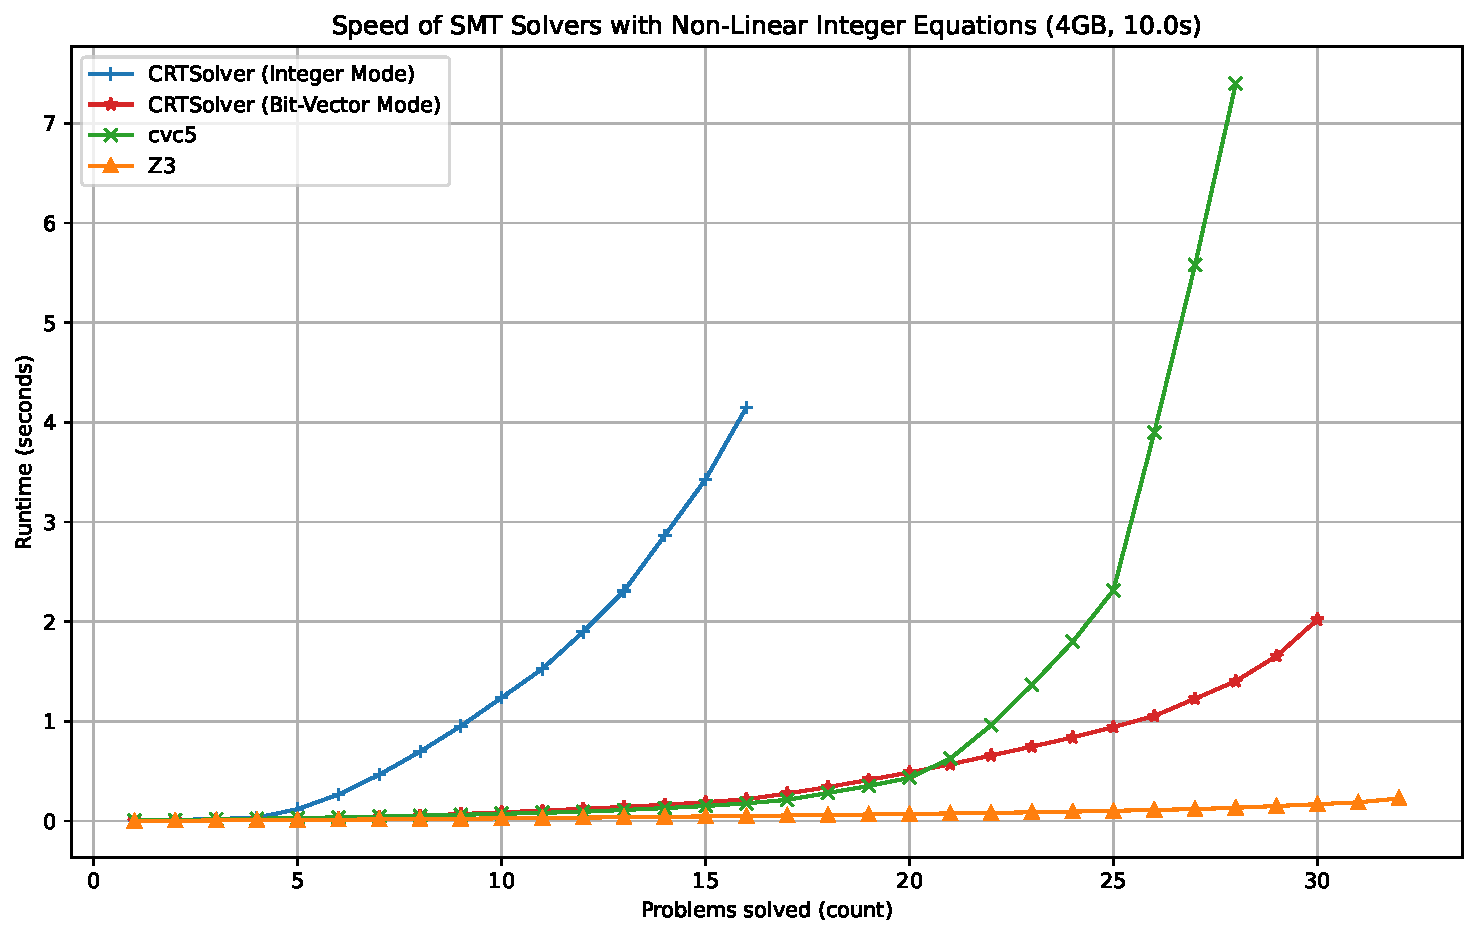
\includegraphics[width=1.0\linewidth]{cactus.pdf}
  \caption{A cactus plot of the results.}
  \label{figure:cactus-plot}
\end{figure*}

These results suggest that there using CRTSolver realistic potential in using CRTSolver in Bit-Vector Mode
as a solver that offers equal or better performance than existing solvers for non-linear
integer equations. However, the Integer Mode of CRTSolver can be safely concluded as having no real potential.
\mbsays{Rewrite when results are available.}


\section{Conclusion}
\label{section:conclusion}

\mbsays{This is in note form, please try to write.  This should not be more than a page.  Half a page is probably about right.}

It works (on the limited set of benchmarks we have tried).

It shows enough promise to be investigated further.
We want to try to implement it in an actual solver.

There are many open questions and possible future directions:
\begin{itemize}
\item{Are there better encodings for solving the modulo sub problems in the BV solver?}
\item{We select primes sequentially, is that the best thing to do or are there better strategies given the encoding, the constants in the problem, how previous candidates have failed, etc.}
\item{How many candidates should be checked, how should they be picked?}
\item{Can the failed candidates be used to improve the modulo sub problems?}
\item{Can this technique be extended to non-equalities ($\not=$), inequalities ($\leq$) and non-polynomial expressions?}
\end{itemize}


%% The declaration on generative AI comes in effect
%% in Janary 2025. See also
%% https://ceur-ws.org/GenAI/Policy.html
\section*{Declaration on Generative AI}
  {\em Either:}\newline
  The author(s) have not employed any Generative AI tools.
  \newline
  
 \noindent{\em Or (by using the activity taxonomy in ceur-ws.org/genai-tax.html):\newline}
 During the preparation of this work, the author(s) used X-GPT-4 and Gramby in order to: Grammar and spelling check. Further, the author(s) used X-AI-IMG for figures 3 and 4 in order to: Generate images. After using these tool(s)/service(s), the author(s) reviewed and edited the content as needed and take(s) full responsibility for the publication’s content. 

\mbsays{We need to fill this out.  I haven't used any generative AI tools.}
 
%% Define the bibliography file to be used
\bibliography{CRTSolver}

%\appendix

\end{document}
